%!TEX root = Thesis.tex
\chapter{State of the Art}
The following chapter covers an overview and analysis of the existent solutions in
the related research areas of web-based third-party applications, which were designed specially for retrieving differet type of sensed data to the user. At the beginning the prominent examples of dashboards platforms are studied and evaluated against the requirements described in the previous chapter with a purpose to clarify their individual capabilities.

\section{?Web of Sensors?}
 Since the thesis is targeted at the creation of a generic user-friendly data stream interaction system and currently every project focused on a specific area of realization and concrete sensor types, such as urban environment\cite{song2010real}. The real-time environmental monitoring portal or geospatial infrastructure for effectively or  efficiently collecting and serving vast field data over the web. Internet based urban environment observation system that can real-time monitor environmental changes of temperature, humidity, illumination or air components in urban area. It provides web-based platform, where end-user can simply monitor urban area in his/her city. In environmental monitoring, the field server for constructing outdoor sensor network is a Web-based field observation device, which detects field environmental parameters and publishes them on Internet in real-time.
\newline
\emph{Smart city}\cite{6588063}tool using information technology and communication (ICT) to help local government to monitoring what currently happened in the city. pplication for monitoring city in single dashboard to help summarize the current condition of city. The architecture system use network sensor consisting of sensor nodes that has
function to capture city condition like temperature, air pollution,
water pollution, traffic situation. Also we can add another information socio-economic situation like public health service, economic indicator, energy supplies, etc. We have successfully developed the prototype of the smart city dashboard the give more accurate information of Bandung City, one of big cities in Indonesia. This study has implemented prototype system of smart city dashboard at Bandung. It consists of network sensor, server, application and also communication protocol which is used for
city monitoring. The summary information of city can be displayed in single view to help people watching, analyzing and action to what being happen at the real-time in the city.
\newline
\emph{Microsoft SensorMap\cite{nath2007sensormap}}has proposed a system to monitor and
present physical sensors in the real world. SensorMap allows owners of sensor networks to register their physical sensors and publish their data on SensorMap. They use GeoDB to store the
sensor network information, DataHub to retrieve the new sensor data to enable real time services, and the
aggregator to summarize sensor data in a specific area to clients.
\newline
 \emph{LiveWeb Portal}\cite{yang2011liveweb} presents the architecture, design, and application of a
sensorweb service portal, where sensorweb is a global observation system for varied sensory phenomena from
the physical world and the cyber world. This system has been used to represent and monitor
real-time physical sensor data and cyber activities from ubiquitous sources. LiveWeb meets its goal of providing an efficient and robust sensor information oriented web service, enabled with real-time data representation, monitoringand notification.LiveWeb has the following properties: the system
enables sensorweb service accessible from anywhere, makes sensor network data readable by
anyone, sensor network sharing, the system make sensor data format transparent to data users, real-time data display suits sensor data properties, an offline alert system strengthens real-time features.
\newline
\emph{Internet of Things}\cite{bendel2013service} where presented a service platform based on the Extensible Messaging and Presence Protocol (XMPP) for the development and provision of services for
Internet of Things(IoT) mainly focusing on the integration of things based on service technologies, scenarios in domains like smart cities, automotive or crisis management require service
platforms involving real world objects, backend-systems and mobile devices. And argued necessary usage of
 XMPP client as protocol for unified, real-time communication and introduce the major concepts of our platform. Based on two case studies we demonstrate real-time capabilities of XMPP for remote robot control and service development in the e-mobility domain.
 \newline
 \emph{Dynvoker Portal}\cite{spillner2008ad} a generic human-driven ad-hoc usage approach, by including rapid service testing and dynamic inclusion of services as plugins into applications. Dynvoker consists of a relatively small application core which can be run as a servlet, a web service or a command-line application. explore method-centric and resource-centric services alike, output forms in various formats or integrate GUI services to provide a richer user experience. The generic design of many parts of Dynvoker has yielded a lightweight architecture which is freely available to any interested person as an open source project

\section{Frontend Development Approaches}
In computer science, the frontend is responsible for collecting input from user and processing it to a backend system and another direction - collecting data from backend, namely sensor data steam, and processing it to the user-friendly interface. Therefore, on the one side, generic frontend has to satisfy architecture requirements from backend, such as: fine-grained distributred structure, cross-platforming, multy-user capabilities; and on the other side, define a dynamic user-friendly interface to a end-user. And to satisfy aforementioned requirements from backend server it is necessary to compare all available web-based applications.
\newline
To retrieve sensor data from different resources in one web-based interface existent next approaches :
\begin{itemize}
 \item portal with portlets,
 \item mashup\footnote{\url{http://www.programmableweb.com/applications}},
 \item HTML5 technology
\end{itemize}
%Portal
Portal technology brings information together from diverse sources in a uniform way. Usually, each information source gets its dedicated area on the page for displaying information (a portlet); often, the user can configure which ones to display. The extent to which content is displayed in a 'uniform way' may depend on the intended user and the intended purpose, as well as the diversity of the content. Very often design emphasis is on a certain 'metaphor' for configuring and customizing the presentation of the content and the chosen implementation framework and/or code libraries\cite{pautasso2008restful,seong2006usability}. In portal technologies end-user can customize number of retrieved data sources, but for that he has to be aware what is it and how to integrate it in portal. User interface in portals have fixed layout, style and location on the web page. To make changes in it, end-user needs to have a deep knowlendge of the system architeture and of whole portal entirely.
 \newline
%Mashup
Mashup is a web page, or web application, that uses content from more than one source to create a single new service displayed in a single graphical interface. The term implies easy, fast integration, frequently using open application programming interfaces (API) and data sources to produce enriched results that were not necessarily the original reason for producing the raw source data. The term mashup originally comes from pop music, where people seamlessly combine music from one song with the vocal track from another—thereby mashing them together to create something new. The main characteristics of a mashup are combination, visualization, and aggregation. It is important to make existing data more useful, for personal and professional use. To be able to permanently access the data of other services, mashups are generally client applications or hosted online\cite{mashup}.
Both commercial products and research prototypes have a broad range of features that simplify a mashups design process, and provide mashups storage and publication. But to customize retrived resources end-user have no option, as use only predefined type and numbers of applications, that was created by application or platform developer. Also Mashup approach is strictly platform- and customer-oriented. It is simply provides stack of tools, by using which user through an user-friendly interface 
The architecture of a mashup is divided into three layers:
 \newline
 \begin{itemize}
\item \emph {Presentation / user interaction:} this is the user interface of mashups. The technologies used are HTML/XHTML, CSS, Javascript, Asynchronous Javascript and Xml (Ajax).
 \newline
\item \emph {Web Services:} the product's functionality can be accessed using API services. The technologies used are XMLHTTPRequest, XML-RPC, JSON-RPC, SOAP, REST.
 \newline
\item \emph {Data:} handling the data like sending, storing and receiving. The technologies used are XML, JSON, KML.
 \newline
 \end{itemize}
Architecturally, there are two styles of mashups: Web-based and server-based. Whereas Web-based mashups typically use the user's Web browser to combine and reformat the data, server-based mashups analyze and reformat the data on a remote server and transmit the data to the user's browser in its final form\cite{bolin2005end}.
 \newline
Mashups and portals are both content aggregation technologies. Portals are an older technology designed as an extension to traditional dynamic Web applications, in which the process of converting data content into marked-up Web pages is split into two phases: generation of markup "fragments" and aggregation of the fragments into pages. Each markup fragment is generated by a "portlet", and the portal combines them into a single Web page. Portlets may be hosted locally on the portal server or remotely on a separate server.
\newline
%HTML5
\section{HTML5 Technology}
To satisfy one of the main requirement about dynamic user-friendly interface, adaptable to any kinf of device, mashup rchitecture should be enhanced with a HTML5 Technology. It is based on various design principles, that truly embody a new vision of possibility and practicality\cite{hickson2011html5}.
\begin{itemize}
\item Compatibility(inharit all previous techniques and standards)
\item Utility
\item Secure by Design(origin-based security model that is not only easy to use but is also used consistently by different APIs.)
\item Separation of Presentation and Content(CSS3)
\item Interoperability(Native browser ability instead of complex JavaScript code; a new, simplified DOCTYPE;simplified character set declaration; powerful yet simple HTML5 APIs)
\item Universal Access(suport users with disabilities by using screen readers; media independence-HTML5 functionallity should work across all different devices and platforms; support for all world languages)
\end{itemize}

\section{Sensor Data}
 Since the thesis is targeted at the creation of a generic user-friendly data stream interaction system and currently every project focused on a specific area of realization and concrete sensor types, such as urban environment\cite{song2010real}. The real-time environmental monitoring portal or geospatial infrastructure for effectively or  efficiently collecting and serving vast field data over the web. Internet based urban environment observation system that can real-time monitor environmental changes of temperature, humidity, illumination or air components in urban area. It provides web-based platform, where end-user can simply monitor urban area in his/her city. In environmental monitoring, the field server for constructing outdoor sensor network is a Web-based field observation device, which detects field environmental parameters and publishes them on Internet in real-time.

 smart city\cite{6588063}tool using information technology and communication (ICT) to help local government to monitoring what currently happened in the city. pplication for monitoring city in single dashboard to help summarize the current condition of city. The architecture system use network sensor consisting of sensor nodes that has
function to capture city condition like temperature, air pollution,
water pollution, traffic situation. Also we can add another information socio-economic situation like public health service, economic indicator, energy supplies, etc. We have successfully developed the prototype of the smart city dashboard the give
more accurate information of Bandung City, one of big cities in Indonesia.
This study has implemented prototype system of smart city dashboard at Bandung. It consists of network sensor, server, application and also communication protocol which is used for
city monitoring. The summary information of city can be displayed in single view to help people watching, analyzing and action to what being happen to city.
 
 LiveWeb\cite{yang2011liveweb}

 robots\cite{bendel2013service}.

 We need to determine types of sensed data:
 \newline
  - data-stream
  \newline
  - data on demand

Many of the Web applications seen today incorporate different patterns to merge
functionality directed toward the end user. This section focuses on the design approaches for portal solutions. 
It addresses the design stage of the solution development process, highlighting the key issues that are specific to portal and application designs.

\section{Summary}
This chapter briefly introduced main approaches for building web-based dashboards by retriving sensed data. Main focus was given to its multy-user usability, adaptive UI design, dynamic content composition. Where portal and mashup technology come into a picture. 
\begin{figure}[!ht]
\centering
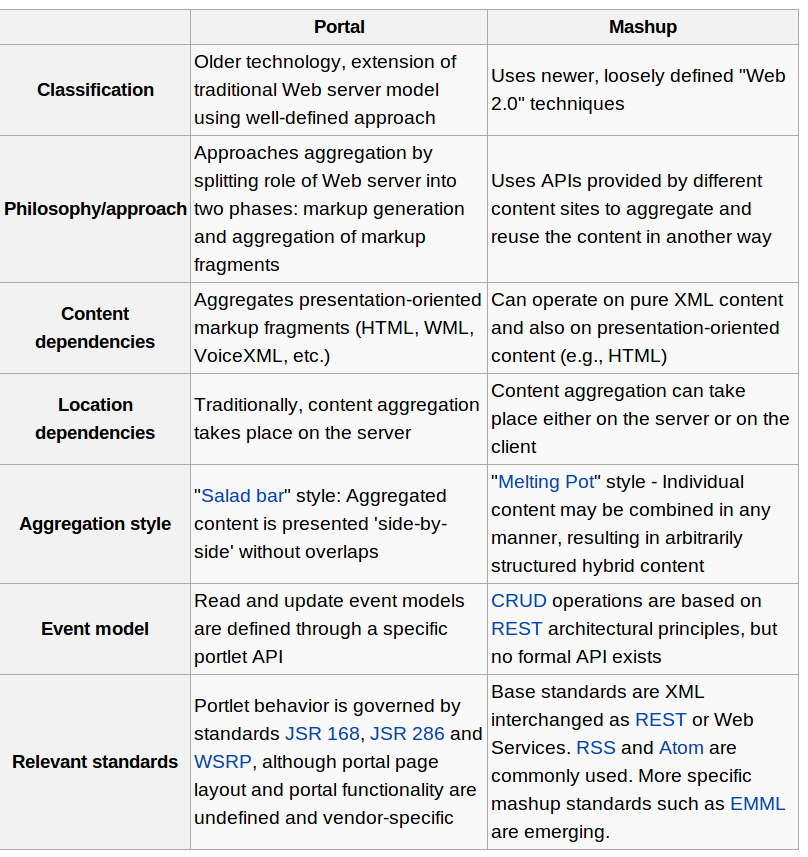
\includegraphics[scale=0.8]{images/MashupVsPortal.png}   
\caption[Comparative Characteristic of Approaches]{Comparative Characteristic}
\label{img:comparative characteristic}                           
\end{figure}
